\section{Gaussian Mixture Model}
\label{sec:gaussian}

\begin{figure}
    \centering
    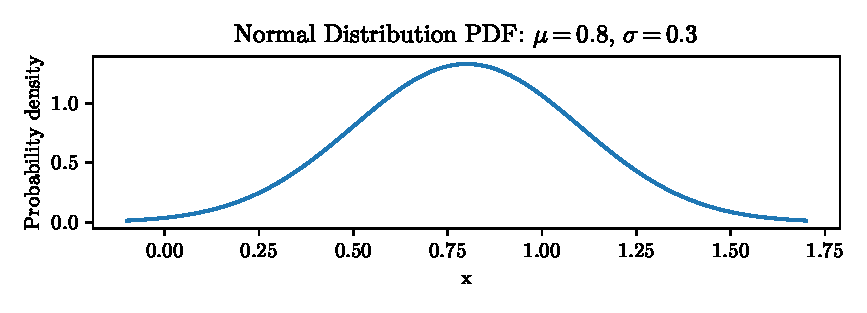
\includegraphics{images/Gaussian/Figure_3.pdf}
    \caption{Gaussian distribution probability density function}
    \label{fig:gauss_pdf}
\end{figure}

The \autoref{fig:gauss_pdf} illustrates a Gaussian distribution probability density function (\gls{pdf}), also known as normal distribution. The peak represents the mean $\mu$, while the spread is determined by the standard deviation $\sigma$. The equation of the \gls{pdf} is the following:

$$
f(x) = \frac{1}{\sigma \sqrt{2\pi} } e^{-\frac{1}{2}\left(\frac{x-\mu}{\sigma}\right)^2}
$$

\paragraph*{}
A Gaussian Mixture Model is a probabilistic model that assumes that the data are generated from a mixture of several Gaussian distributions. Depending on the parameters of a Gaussian distribution (mean and variance) on each axis (Features), the data generated from it in the $\gls{sym:feats}$-dimensional space will have a shape that resembles an ellipsoid with a center and an orientation.


\subsection{Training}
\label{sec:gauss_train}
As anticipated, the assumption is that every cluster has a normal \gls{pdf} on each axis. So, for each feature, the total \gls{pdf} is a superposition of $k$ normal \gls{pdf}. 
The algorithm used to train the model is the Expectation Maximization (\gls{em}) algorithm. This is a generalization of the k-means algorithm that allows to find the centroids (means), the covariance matrices of the clusters, and their weights. Unlike the k-means, the \gls{em} is a soft clustering algorithm, meaning that each point is assigned to each cluster with a probability, instead of being assigned to a single cluster.
The \gls{em} algorithm is an iterative algorithm that aims to find the parameters that maximize the \gls{glo:likelihood}.

\subsection{Selecting the number of clusters}
\begin{figure}[htbp]
    \centering
    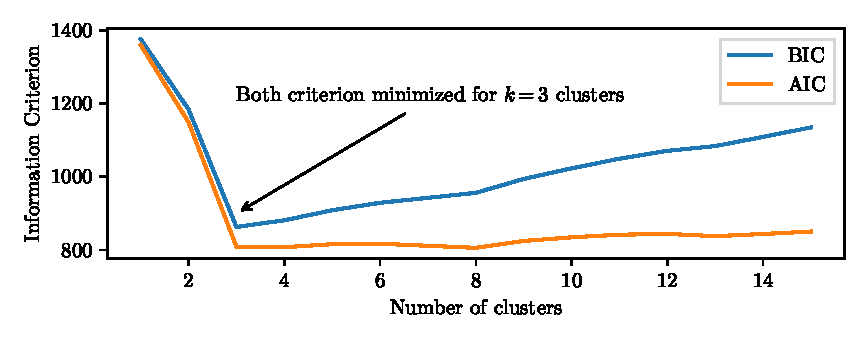
\includegraphics{images/Gaussian/Figure_1.pdf}
    \caption{Criteria for selecting the number of clusters}
    \label{fig:gauss_criterion}
\end{figure}
In \autoref{sec:gauss_train} we have seen that the \gls{em} algorithm needs to know in advance the number of clusters $k$ to train the model. To select the best $k$ we could use the same criteria used for the k-means, that is the elbow method or the silhouette score. But, since the \gls{em} is most suitable for ellipsoids-shaped clusters of very different sizes, it is better to avoid those metrics that work best with spherical clusters. Instead, we can use the \gls{aic} or the \gls{bic} criteria, which are functions of the size $m$ of the training dataset, the number $p$ of parameters, and the max value of \gls{glo:likelihood} $\hat{\mathcal{L}}$.

\begin{equation}
    \begin{matrix}
        \gls{aic} &=& 2p - 2 \ln(\hat{\mathcal{L}}) \\
        \gls{bic} &=& p \ln(m) - 2 \ln(\hat{\mathcal{L}})
    \end{matrix}
    \label{eq:aic_bic}
\end{equation}

Both the criteria in \autoref{eq:aic_bic} penalize the models with a large number of parameters, they usually select the same model, but if they select different models, the \gls{aic} tends to select the most accurate model.

Considering, as an example, the same dataset used in \autoref{fig:dbscandata}, and running the \gls{em} algorithm with different values of $k$, we obtain the results shown in \autoref{fig:gauss_criterion}. As expected the \gls{aic} and the \gls{bic} criteria select the same model, that is the one with $k=3$.

\subsection{Evaluation of a new instance}
\label{sec:gauss_eval}
\begin{figure}
    \centering
    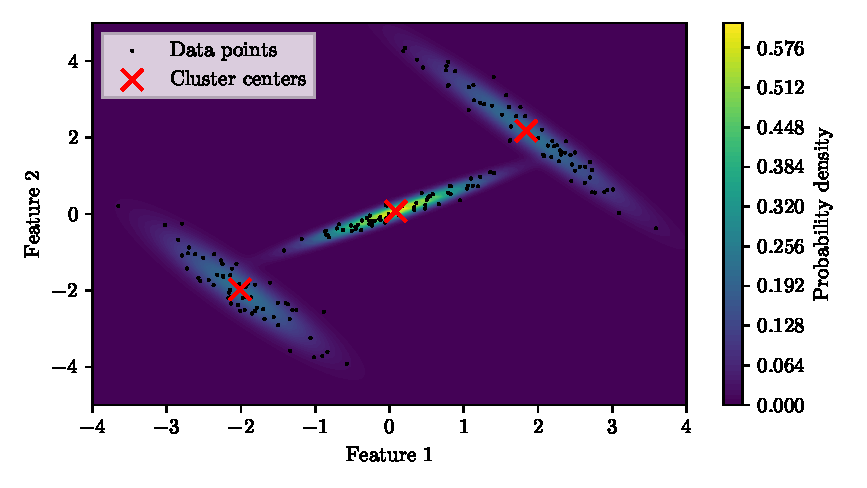
\includegraphics{images/Gaussian/Figure_2.pdf}
    \caption{Trained Gaussian Mixture Model}
    \label{fig:gauss_example}
\end{figure}
Once the model is well trained, we can use it to evaluate a new instance. The \autoref{fig:gauss_example} shows the result of the training of the \gls{gmm} on the example dataset. The ellipsoids represent the clusters, the size of the ellipsoids is proportional to the weight of the cluster, while the orientation and the size of the ellipsoids are determined by the covariance matrix of the cluster. 

The \texttt{pyhton} implementation of the \gls{gmm} used in this project is the one provided by the \texttt{sklearn} library. It has an attribute called \texttt{score\_samples} that returns the log value of the \gls{pdf} of the samples.
The bigger the value, the more likely it is to be inside a cluster. 
To maintain the same philosophy of the other algorithms, we can take the negative value of \texttt{score\_samples} as a metric to evaluate the novelty of a new instance. 

\subsection{Selecting the threshold}
As said for K-means, and \gls{dbscan}, a threshold will be needed to decide if the new instance is novel or not. If, as supposed for now, the scenario is that the training dataset is composed only of normal instances, then the threshold can be selected by looking at the distribution of the novelty metric on the training dataset, and selecting a value slightly higher than the maximum value for the training dataset.

If the scenario is that the training dataset is composed of both normal and anomalous instances sampled at constant intervals, and the ratio between normal and anomalous instances is Known, then \gls{gmm} enables us to select the threshold in a more sophisticated way.

Suppose for example that $1\%$ of the training dataset is anomalous, since the model gives us the \gls{pdf} of the samples, we can compute the threshold as the $1\%$ percentile of the \gls{pdf} of the training dataset. This will ensure that the $1\%$ of the training instances will be classified as anomalous. If the model is correct, also future evaluations will have the same ratio of anomalous instances.

\subsection{Totally unsupervised approach}
\label{sec:gauss_unsupervised}
Another advantage of the \gls{gmm} is that it can be used in a totally unsupervised way. This can be done using the variation called Bayesian Gaussian Mixture Model \gls{bgmm}. This variation is able to assign $0$ as 
weight to some clusters, meaning that those clusters are not used to generate the \gls{pdf} of the samples. In this case, we can set the number of clusters as high as the size of the training dataset, and the \gls{bgmm} will select the best number of clusters to use to generate the \gls{pdf} of the samples. 

\subsection{Limitations of \gls{gmm}}
The main limitation of the \gls{gmm} is that it is not able to identify clusters with arbitrary shapes.

If the data are not shaped like some ellipsoids, the model can approximate the data anyway, splitting the clusters into smaller ellipsoids. For our purposes of novelty detection, this is not a limitation.

The complexity of the algorithm is $\mathcal{O}(kmF^2+kF^3)$, where $k$ is the number of clusters, $m$ is the number of samples, and $F$ is the number of features \citepage{hands-on-geron2022}{281}. This means that the algorithm is not scalable to a large number of features, but it is scalable to a large number of samples.
For our purposes, it's more important to have an algorithm that is fast to evaluate a new instance, than an algorithm that is fast to train.